
In this experiment we measure the characteristic $T_1$ time of the qubit~\cite{Klimov2018}.
This is the first experiment that cannot be considered calibration since no control parameter gets changed, but rather we are trying to understand better the qubit so we can talk of pure \textit{characterization}.

The experiment is easy to understand and follow: we first excite the qubit with a \pipulse, then wait some time and measure. 
If the waiting time is zero, then we expect to measure the amplitude of the excited state $\ket 1$, if the wait time is $\infty$ then we expect the qubit to have completely relaxed to $\ket 0$ before the measurement.
For intermediate wait times, we have an time-exponentially decaying probability of relaxation so, for a sufficiently large number of shots, we expect to see the same shape for the measured amplitude.

Therefore, we can fit the obtained curve with a simple exponential:
\begin{equation}
    y = p_0 - p_1 e^{-\frac{x}{T_1}}
\end{equation}

In \cref{fig:t1_experiment} a real $T_1$ experiment is shown.
\begin{figure}[ht]
    \makebox[\textwidth][c]{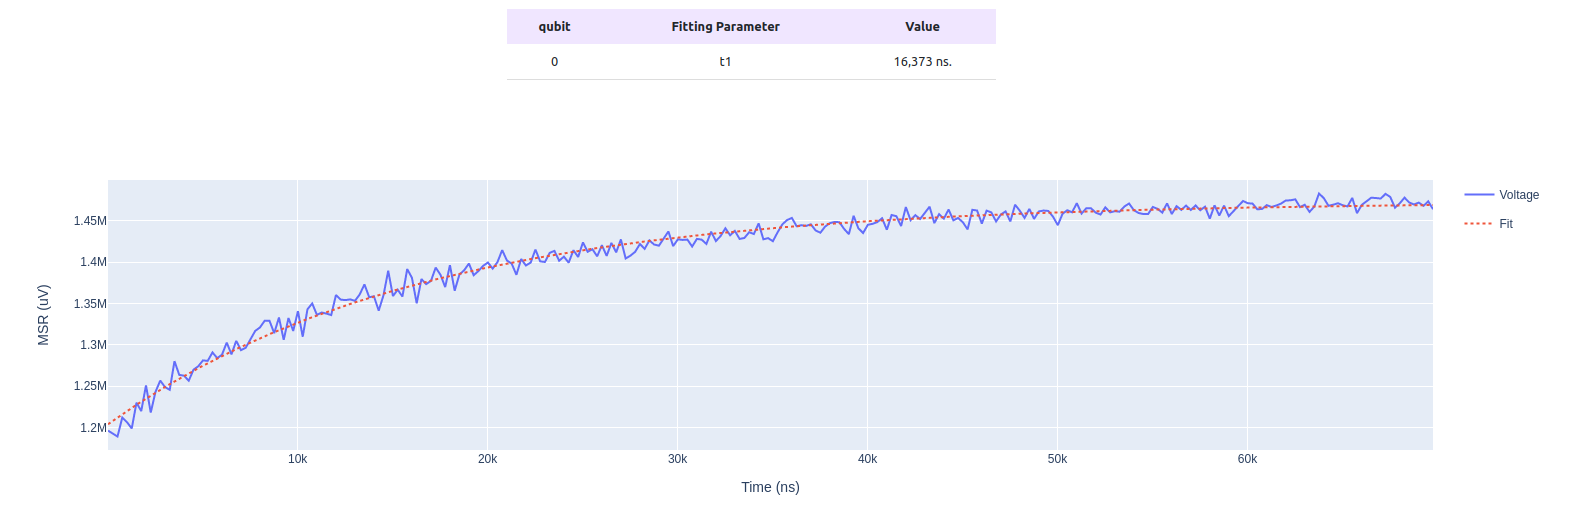
\includegraphics[width=1.3\textwidth]{characterization/figures/t1_16mus.png}}
    \caption{Plot of a T1 experiment.}
    \label{fig:t1_experiment}
\end{figure}


\experimentrecap
{T1 measurement}
{qubit characterization}
{characteristic relaxation time $T_1$}
{a \pipulse is sent to the qubit through the drive line, after a variable wait time we perform a measurement. We plot the measurement amplitude against the waiting time and fit the curve with a simple exponential function. The decay constant will be $T_1$}
